\documentclass[a4paper,11pt]{jsarticle}


% 数式
\usepackage{amsmath,amsfonts}
\usepackage{bm}
% 画像
\usepackage[dvipdfmx]{graphicx}

%ハイパーリンク
\usepackage[dvipdfmx]{hyperref}
\usepackage{pxjahyper} % (u)pLaTeXのときのみかく
\hypersetup{%
 setpagesize=false,%
 bookmarks=true,%
 bookmarksdepth=tocdepth,%
 bookmarksnumbered=true,%
 colorlinks=true,%
 anchorcolor=black,
 linkcolor=black,
 pdftitle={},%
 pdfsubject={},%
 pdfauthor={},%
 pdfkeywords={}}

\title{SolidWorks2021による3次元CAD}
\author{からくりサークル有志}
\date{\today}

\begin{document}
\maketitle
\clearpage
\tableofcontents
\clearpage

\section{はじめに}
この資料はSOLIDWORKS2021を初めて使う人向けに書いたものであることをご理解いただきたい.また,文字による説明のみであるため,とっつきにくさを感じるかもしれないが,説明はかなり詳しく書いたつもりなので,なんとかなるはずである.
\subsection{前提知識}
名称などは覚える必要はない.読み進める途中で知らない名称が出てきたとき,ここに返ってくるぐらいの気持ちで大丈夫である.
\begin{figure}[h]
 \begin{center}
  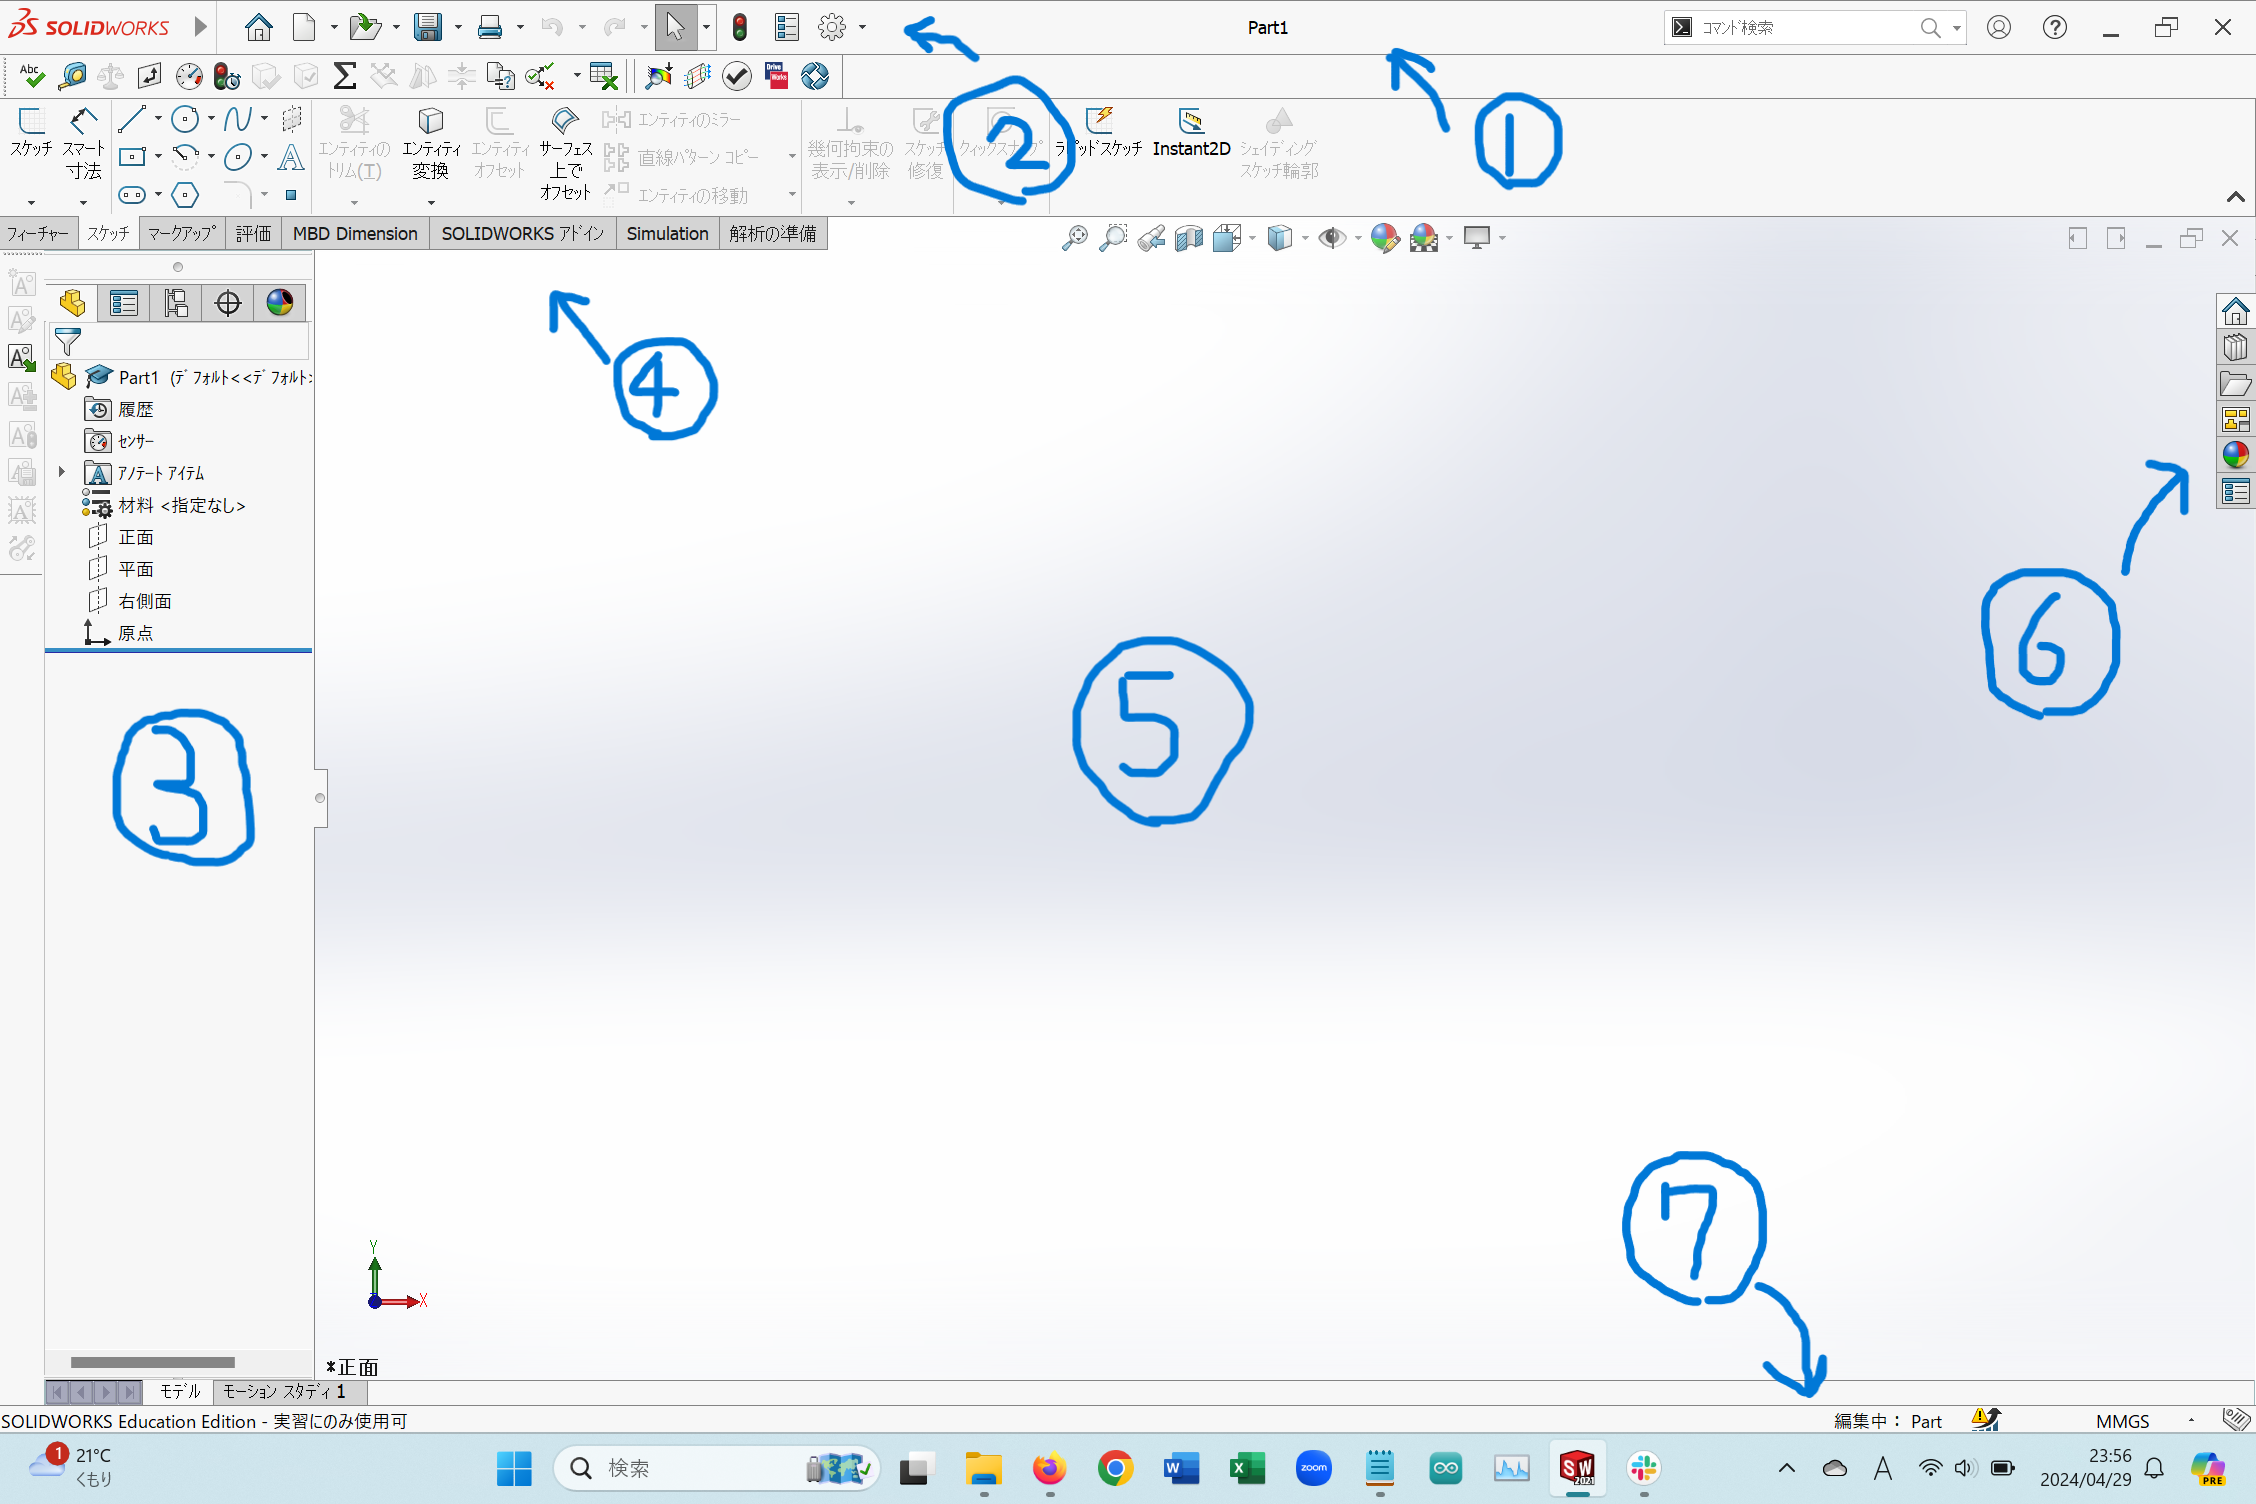
\includegraphics[width=100mm]{solidworks_menu1.png}
  \caption{画面の構成(覚える必要はない)}
 \end{center}
\end{figure}
\begin{table}[h]
\centering
\begin{tabular}[t]{|c|c|}
 ①タイトルバー & 画面最上部.作業中のファイル名が表示される \\
 ②プルダウンメニュー(メニューバー) & タイトルバーと同じ欄にあるメニュー \\
 ③Feature Manager デザインツリー & モデルの構成や作業過程を表示する \\
 ④ツールバー & スケッチやフィーチャー編集,使うことになる \\
 ⑤グラフィックス領域 & 作業領域\\
 ⑥タスクパネル & ToolBoxを使う際に用いる \\
 ⑦ステータスバー & メッセージや作業の情報が表示される \\
\end{tabular}
\end{table}
\clearpage
\subsubsection{各種コマンド}
コマンドは知っておくと操作がかなり楽になるため,この節は一見の価値があるだろう.
\begin{itemize}
 \item 'Del':選択したものを削除
 \item '右クリック':メニューを表示(大体の操作をここで表示されるメニューから行える)
 \item 'F':モデルを画面にフィット
 \item 'Ctrl + N':新規ファイルの作成
 \item 'Ctrl + S':ファイルの保存\footnote{5.7を参照}
 \item 'Ctrl + クリック':複数選択
 \item 'ピンチアウト/イン':モデルの拡大/縮小
 \item 'Ctrl + 十字キー':モデルの移動
 \item '十字キー':モデルの回転
 \item 'Shift + 十字キー':モデルを90[deg]ずつ回転
 \item 'Ctrl + 1 - 8':各種グローバル座標をもとにした視点変更(特にCtrl + 7はモデルが見やすくなるため多用することになるだろう)
 \item 'Enter':直前の作業を続ける
\end{itemize}
\section{スケッチ}
まず2次元のスケッチを描き,そのスケッチをもとにフィーチャー編集を行うことで,3次元モデルを作るというのが基本的な流れである.
\subsection{立体成型用のスケッチ}
\begin{enumerate}
 \item ファイルの新規作成から部品を選択.
 \item スケッチ平面の選択.
 \begin{enumerate}
  \item Feature Manager デザインツリーの'正面','平面','右側面'の中からスケッチしたい平面を選択.
  \item ツールバーよりスケッチタブを選択.
  \item 更にスケッチを選択.
 \end{enumerate}
 \item 描きたいスケッチを描く(四角形を描く際は矩形中心を選ぶと描きやすい).
 \item スケッチの完全定義.
 \begin{enumerate}
 \item 幾何拘束の追加.
  \begin{enumerate}
   \item '原点'と'スケッチの点(適切な点)'を複数選択(Ctrl+クリック).
   \item Feature Manager デザインツリーの表示が変わったことを確認.
   \item Feature Manager デザインツリーから'一致'を選択(これにより,選択した点同士が固定される).
   \item 必要に応じ,幾何拘束を追加する.
  \end{enumerate}
 \item 寸法の追加.
  \begin{enumerate}
   \item ツールバーのスケッチタブ内のスマート寸法を選択.
   \item 辺を選択し,長さを定義する(これにより長さが固定される).
   \begin{itemize}
    \item スマート寸法を用いる際,「フィーチャーの取り付けに失敗しました」と言われることがある.そうなったときは,その状態のまま適当な面を選択し,適当に寸法を追加する.その後,寸法線を選択し'Delキー'で消すと良い.
   \end{itemize}
  \end{enumerate}
 \end{enumerate}
 \item 最後に,スケッチした線すべてが,黒くなっていることを確認(フィーチャー編集へ続く).
\end{enumerate}
\subsection{穴あけ用のスケッチ}
この節では,すでに3次元のモデルがあることを前提としている.
\begin{enumerate}
 \item スケッチする面の選択.
 \begin{enumerate}
  \item モデルのスケッチしたい面を右クリック.
  \item 表示されたメニューからスケッチを選択.
 \end{enumerate}
\item 中心線を引く(角パイプの場合).
\begin{enumerate}
 \item 直線を引く(ダブルクリックで'直線を引く'を終了できる).
 \item 直線を選択し,作図線,無限遠にチェックをつける.
 \item 幾何拘束'中点'を追加(角パイプの短辺と,直線を選択).
\end{enumerate}
 \item 穴あけ用の円(3.2mm)をスケッチし幾何拘束を定義する.
 \begin{enumerate}
  \item 円をスケッチ.
  \item スケッチした円の中心と,中心線を'複数選択'する(中心点1つと線を選択).
  \item 幾何拘束'一致'を選択.
  \item (円が複数ある場合)同一スケッチ上の同一径の円周,全てを複数選択.
  \item 幾何拘束'等しい値'を選択(一つの円の直径を定義すると選択した他の円もその直径で定義される).
 \end{enumerate}
\item 最後に,スケッチした線すべてが,黒くなっていることを確認(フィーチャー編集へ続く).
\end{enumerate}
\subsection{角パイプのスケッチ}
このサークルでは主に9x9mm角パイプ(肉厚1.2mm),12x12mm角パイプ(肉厚1.5mm)が用いられる.\\
角パイプのスケッチにはエンティティのオフセットが便利である.
\begin{enumerate}
 \item 欲しい角パイプの外側の正方形をスケッチし,完全定義する(9mmの正方形 or 12mmの正方形).
 \item エンティティオフセット.
 \begin{enumerate}
  \item ツールバーのスケッチタブから,エンティティオフセットを選択
  \item パラメータを角パイプの肉厚分に変える
  \item 寸法の追加反対方向チェーン選択にチェックをつける
  \item スケッチ線を選択(選択すると黄色い線で予測してくれる)
 \end{enumerate}
 \item スケッチ終了(フィーチャー編集から任意の長さの角パイプを得る).
\end{enumerate}
\subsection{その他の知識}
\subsubsection{直線/円形パターン}
規則正しくスケッチが並ぶ際に使用する.\\
モーターなど既成品のネジ穴を定義する際に用いる.
\subsubsection{幾何拘束}
幾何拘束には多くの種類がある.使用頻度の高いものを紹介する.\\
\begin{table}[h]
\centering
\begin{tabular}[t]{|c|c|}
 水平& 水平線の定義\\
 鉛直& 鉛直線の定義\\
 一致& 点と点/線を複数選択し一致させる\\
 等しい値& 円の直径を揃える際に有用である\\
\end{tabular}
\end{table}
\subsubsection{エンティティ変換}
スケッチ平面の奥の面の正射影をスケッチとして用いたい場合に使用する.
\subsubsection{完全定義}
完全定義とは,スケッチがグローバル座標から見て,スケッチが定義された状態のことを指す.完全定義されたスケッチかどうかの見分け方は,2つある.\\
 1つ目は,Feature Manager デザインツリーでスケッチ名を表示させたとき,スケッチ名の前に''(-)''このマークがあるかないかという方法である.''(-)''があるときそのスケッチは完全定義されていないものである.\\
 2つ目は,スケッチ編集を開いた際の,スケッチ線の色で確認する方法である.スケッチ線が青い場合その線は定義されていないことを指す.スケッチ線が全て黒くなっていればそのスケッチは,完全定義されていることを指す.
\paragraph{なぜ完全定義をするのか}
以下に示すのは単に意見である.\\
「完全定義をしなくても,スケッチ編集さえ開かなければ,モデルは定義されているし困ることは何もないのに,何故完全定義しなければならないのか.」という問を持つことは至極当然のことであろう.私もSOLIDWORKS2021を触り始め,先輩に完全定義しろと言われたとき,同様の疑問を持ったことを覚えている.\\
 完全定義に必要なもの,それはスケッチの寸法の追加と,原点との関係の定義である.スケッチに寸法を追加することの必要性は言うまでもないだろう.では何故,原点との関係性を定義しなければならないのか.それは,グローバル座標系でスケッチを定義するためである.原点との関係が記述されていないスケッチは,ローカル座標系でしか定義されていないものとみなすことができる.これは言い換えると,座標系のとり方で,見え方が変わってしまうものである.設計図が一意に定まらないものを設計とは言えないため,原点との関係を記述し,完全定義をする必要があるのだ.
\subsubsection{線の色}
\begin{table}[h]
 \centering
\begin{tabular}[t]{|c|c|}
 青色& スケッチ線(未定義)\\
 水色& 選択している線\\
 黒色& スケッチ線(完全定義)\\
 黄色& 重複定義(幾何拘束や寸法の追加で過剰に定義していることを示す)\\
\end{tabular}
\end{table}
\section{3次元モデルの作成}
この節では,作成したスケッチから3次元モデルを作成する方法をいくつか示す.
\subsection{押し出しボス/ベース}
3次元モデルを得る際,最も使うことになるのが'押し出しボス/ベース'だろう.
\subsubsection{方法}
\begin{enumerate}
 \item Feature Manager デザインツリーから,スケッチを選択.
 \item ツールバーでフィーチャータブを選択し,押し出しボス/ベースを選択.
 \item ブラインドが選択されていることを確認し,寸法を追加.
 \item チェックマークをクリック.
\end{enumerate}
\subsubsection{その他の使い方}
押し出しボス/ベースでは,前述したこと以外の用い方もできる.その一つが薄型フィーチャーである.
枠だけのスケッチに対して押し出しボス/ベースから薄型フィーチャーを選択することで,肉厚を与えつつ,3Dモデルを作成することができる.\\
(注)この操作により,パイプ形状のモデルの作成は容易に行える.しかし,スケッチ内に肉厚部分の定義がないものとなってしまう.
これは,あまりよろしくないことなので,この操作を用いるのは最終手段だと思ってほしい(エンティティのオフセットを使い肉厚を定義したスケッチからモデルを作ること).\\
また,輪郭選択というものもある.これはスケッチ内に閉じた領域が2つ以上ある場合に選択が可能なものである.努めて使うものではないため,頭の片隅においてあれば良い.
\subsection{押し出しカット}
3次元モデルに穴を開ける際に用いることになる.また,モデルの余分な部分をカットする際にも用いる.
\subsubsection{方法}
\begin{enumerate}
 \item Feature Feature Manager デザインツリーから,スケッチを選択.
 \item ツールバーでフィーチャータブを選択し,押し出しカットを選択.
 \item 全貫通が選択されていることを確認する.
 \item 'チェックマーク'をクリック.
\end{enumerate}
\subsubsection{その他の使い方}
前述した,輪郭選択が押し出しカットにもある.押し出しカットの輪郭選択については,一度に大量の穴を開けようとした際に,システム側から輪郭選択を使うよう求められることがある.求められたときに,どのように操作すればよいか知っておく程度でよい.
\paragraph{方法}
\begin{enumerate}
 \item Feature Manager デザインツリーから押し出しカットのモードであることを確認.
 \item Feature Manager デザインツリーから輪郭選択を選択.
 \item 輪郭選択を選んだ際に出てきた枠が青くなっていることを確認.
 \item スケッチ内でカットしたい領域を選択する.
 \item 'チェックマーク'をクリック.
\end{enumerate}
\subsection{その他のフィーチャー編集}
\subsubsection{回転ボス/ベース}
断面と,回転軸のスケッチを定義することで使える.\\
球形のモデルを作成する際に用いる.
\subsubsection{フィレット}
作成したスケッチの角,モデルの角に対して行える操作.\\
モデルの角を丸くしたり,面取りをする際に用いる.
\subsubsection{参照ジオメトリ→平面}
曲面に対してスケッチをする際に使用する.\\
新たな面を定義できるため,便利なときがある.
\subsubsection{カーブ→分割ライン}
モデルの平面を,平面内のスケッチ部分で分割できる.\\
フィールドのCADを作成するとき,フィールド内のラインを再現するために用いる.
\section{アセンブリ}
今までの作業を経て部品が揃って来たら,ついにアセンブリのときである.
\subsection{方法}
\begin{enumerate}
 \item ファイルの新規作成からアセンブリを選択.
 \item 構成部品の挿入.
 \begin{enumerate}
  \item ツールバーのアセンブリタブから構成部品の挿入を選択
  \item Feature Manager デザインツリーの'参照'をクリック
  \item 挿入する部品を選択し'OK'をクリック
 \end{enumerate}
 \item 合致.
 \begin{enumerate}
  \item ツールバーのアセンブリタブから合致を選択
  \item 各種合致を選択する(合致に関しては後に説明)
 \end{enumerate}
 \item 必要な分だけ部品の挿入と合致を繰り返す.
\end{enumerate}
\subsection{合致}\label{gatti}
合致は,アセンブリをする際に最も重要なものである.\\
合致によって,挿入したパーツ同士の関係を定義できるのであるが,適当に合致をすると,現実世界ではありえない固定のされ方をした設計となることがある(ネジがないのに固定されている等)ため,慎重に行う必要がある.しかし,うまく合致を行うことで,アセンブリ内で実際の動きを再現させることができる.以下に主に使われる合致と,使用例を示す.
\clearpage
\begin{table}[h]
 \centering
\begin{tabular}[t]{ccc}
\hline
 一致& 面-面/軸線-軸線& \begin{tabular}{c}
			 基本的にこの合致を使う\\
			 面同士が同じ面で接するようにする\\
			 軸線同士が一直線に並ぶようにする\\
			\end{tabular}\\
\hline
 距離(詳細設定タブ)& 面-面& \begin{tabular}{c}
			     主にエアシリンダーなどのストロークが\\
			     決まったものに対して用いる\\
			    \end{tabular}\\
\hline
\end{tabular}
\end{table}
上に示した合致以外にも様々な合致がある.上に示せなかった合致はみなさんがSOLIDWORKSに慣れてきてから,自分で試して見ると良いだろう.
\subsection{アセンブリにおける注意}
ネジや電送など,CADに反映されない部品を考慮し設計をする必要がある.
\subsection{その他の操作}
\subsubsection{パーツを開く}
アセンブリファイルから,パーツのファイルを開くときに使う.\\
開きたいパーツを'右クリック'表示されるメニューから,部品を開くを選択.
\subsubsection{SOLIDWORKS Toolbox}
ギアや,ネジなどのパーツをCADに反映させたいとき用いる.
\begin{enumerate}
 \item アセンブリファイル内であることを確認.
 \item タスクパネルのデザインライブラリのToolboxを選択.
 \item '今アドイン'を選択し,Toolboxが開かれるのを待つ.
 \item JISのフォルダを開き,欲しいパーツをドラッグ&ドロップ(グラフィックス領域内へ).
 \item 各種定義をFeature Manager デザインツリーから行う.
\end{enumerate}
\subsubsection{評価}
ツールバーの評価タブ内の'干渉認識','測定'は有用である.
特にCADから寸法線を得る際には,スマート寸法などではなく,'測定'使うことをお薦めする.
\begin{itemize}
 \item 干渉認識:アセンブリ時に使用して,無理のない設計か確かめる際に用いる.
 \item 測定:辺-円周及び辺-辺を選択し,長さを得る.
\end{itemize}
\section{+α}
\subsection{材料の設定}
パーツファイルのFeature Manager デザインツリーで材料の定義を行うことで,ある程度の質量が求められる.質量を考慮し設計することは重要なことなので,面倒だが毎回定義することをお薦めする.また,材料を定義することで,重心計算も可能となる.\\
参考までに,アルミ角パイプの場合,質量密度の欄を2375とすると良い.
\subsection{外観の設定}
フィールドのCADを作成する際に必要となる.
\begin{enumerate}
 \item タスクパネルの'外観,シーン,デカル'を選択.
 \item 色と書かれた'図'を選択.
 \item Feature Manager デザインツリーから色を指定できる.
\end{enumerate}
\subsection{グラフィックス領域上部のメニューについて}
主に視覚的な変化をもたらすことができる.
\begin{itemize}
 \item 目のアイコンを開き,一時的な軸を表示させると,ネジ穴の合致がしやすくなる.
 \item グラフィックス領域内右上のバツじるしを選択することで,表示中のファイルを閉じることができる.
\end{itemize}
\subsection{Pack and go}
SOLIDWORKSのファイルを誰かに送る際,一度Zipファイルに圧縮する必要がある.
この圧縮作業はSOLIDWORKS側から行わないと,エラーが起きる.このとき用いるのが'Pack and go'である.
\begin{itemize}
 \item メニューバーのファイルから'Pack and go'を選択.
 \item '単一フォルダに平坦化'にチェックをつける.
 \item '参照'から,保存先のフォルダを指定する(フォルダを新規作成しそこを指定すると良い).
 \item '保存'をクリック.
\end{itemize}
\subsection{stlファイルへの変換}
3Dプリンターを用いる際に必要となる.
\begin{enumerate}
 \item 3Dプリントを行う際,穴の直径に補正をかける(大体+0.2mm).
 \item メニューバー保存マークを展開.
 \item 指定保存を選択.
 \item 名前をつける際に,拡張子を.stlに変更し,コピーを指定保存して続行を選択.
 \item 保存する.
\end{enumerate}
\subsection{Dxfファイルのエクスポート}
レーザープリンターを用いる際に必要となる.
\begin{enumerate}
 \item プリントする面を右クリック.
 \item Dxfにエクスポートを選択.
\end{enumerate}
\subsection{ファイルの名前について}
SOLIDWORKSではファイルの名前がかぶると,エラーが起きることがある.そのため,ファイルの名前は個性的なものであることが望ましい.\\
良くない名前の例
\begin{itemize}
 \item part1
 \item body01
\end{itemize}
\end{document}
